\documentclass[conference]{IEEEtran}
\usepackage{amsmath,booktabs,graphicx,url}
\title{Safe Alone, Unsafe Together: Minimal Dynamic Incompatibility in SG-to-GFL Replacement Portfolios}
\author{TX4 research campaign}
\begin{document}
\maketitle
\begin{abstract}
Replacement safety is not necessarily compositional. In a frozen IEEE-39
phasor-domain model, four local SG-to-GFL replacements form an unstable
portfolio although each of its fifteen proper subsets is stable. We build one
all-SG network kernel and four local replacement models, then predict the
four-bus verdict before full-order reveal. The prediction is exact over all
16 portfolios. A classical contextual-return factorization identifies the
collective closure responsible for the failure, and a nonlinear phasor-domain
load-pulse test preserves the stable/unstable/stable ordering. A 512-portfolio
benchmark is deliberately negative: accuracy is 77.15\%, with 116 false-safe
cases and no exact blocker-family recovery. The contribution is therefore a
scoped model-specific mechanism and prediction package, not a universal
portfolio predictor.
\end{abstract}

\section{Industrial question}
As synchronous generation is replaced by grid-following converters, a plan
that checks each replacement alone may miss a collective dynamic failure.
The planning question is discrete: which finite set of local replacements is
the first incompatible set, while load, dispatch, and network remain fixed?

This question is deliberately narrower than a generic grid-strength study.
The object being tested is a finite replacement portfolio under one frozen
policy, not an uncertainty distribution. The evidence is consequently
reported as an exact finite census and as a preregistered blind test.

\begin{figure}[t]
\centering
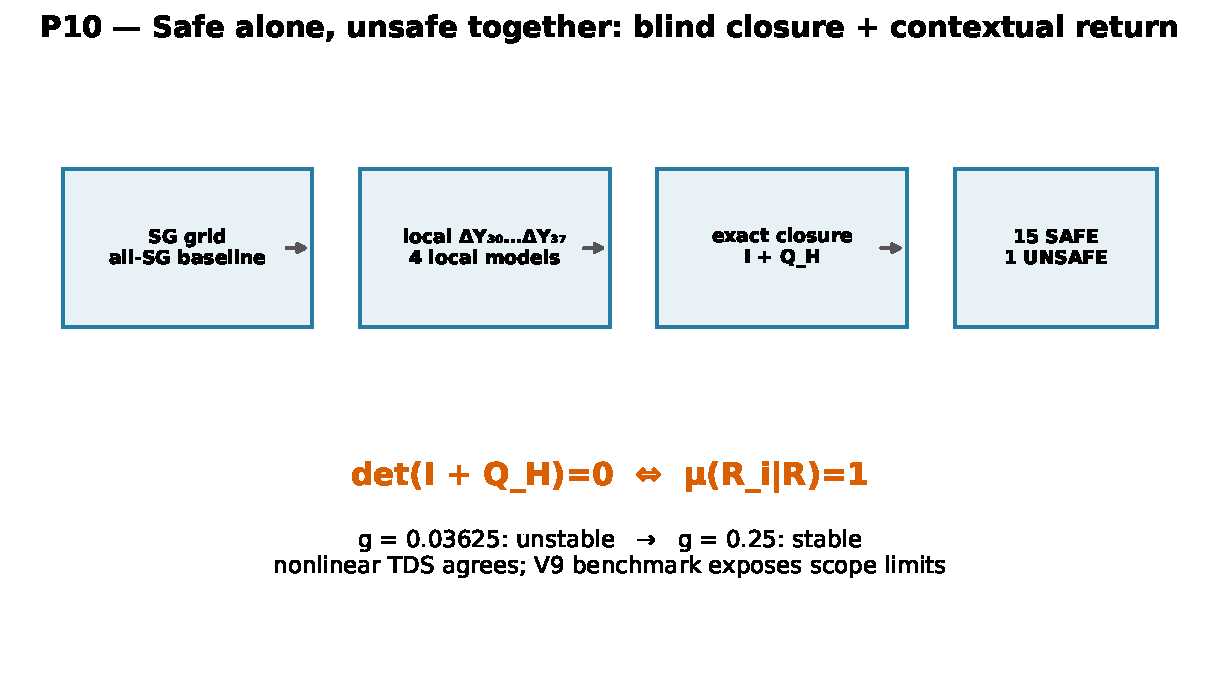
\includegraphics[width=.95\columnwidth]{../../../figures/tx4_blind_prediction/P10_graphical_abstract.pdf}
\caption{Campaign logic: local replacements are composed through a common network closure, then checked against full-order dynamics.}
\label{fig:abstract}
\end{figure}

\section{Frozen model and witness}
The IEEE-39 phasor-domain DAE uses the frozen TX4 synchronous-machine, AVR,
and ten-state GFL semantics. At P4,
$(g,k,t,h)=(0.03625,1.425,1.5,1)$, H4=$\{30,33,35,37\}$ has
$\alpha=+0.127006$ s$^{-1}$ at 0.622280 Hz. Every proper subset is stable;
the four 7-of-8 predecessors have alpha values -0.204688, -0.175508,
-0.167856, and -0.203009 s$^{-1}$.

The four candidate buses are 30, 33, 35, and 37. The full-order test resolves
the equilibrium before extracting the spectrum; the reduced test uses the
same operating-point-matched local substitutions. This common setup matters
because a portfolio verdict can otherwise be confounded with a different
dispatch or initialization.

\section{Reduced closure}
Let $T_0(s)$ be the all-SG network port and
$K=E^TT_0^{-1}E$. Local substitutions give $D_S$ and
$M_S=D_SK_{SS}$. After diagonal normalization,
$Q_S=(I+D_SK_d)^{-1}D_SK_o$. This is an exact determinant factorization
under regularity assumptions; the algebra is classical.

The representation is useful because it reuses one network kernel and changes
only local device terms. It is not a claim that a reduced determinant has the
same spectral-abscissa ordering for every portfolio or operating point.

\begin{figure}[t]
\centering
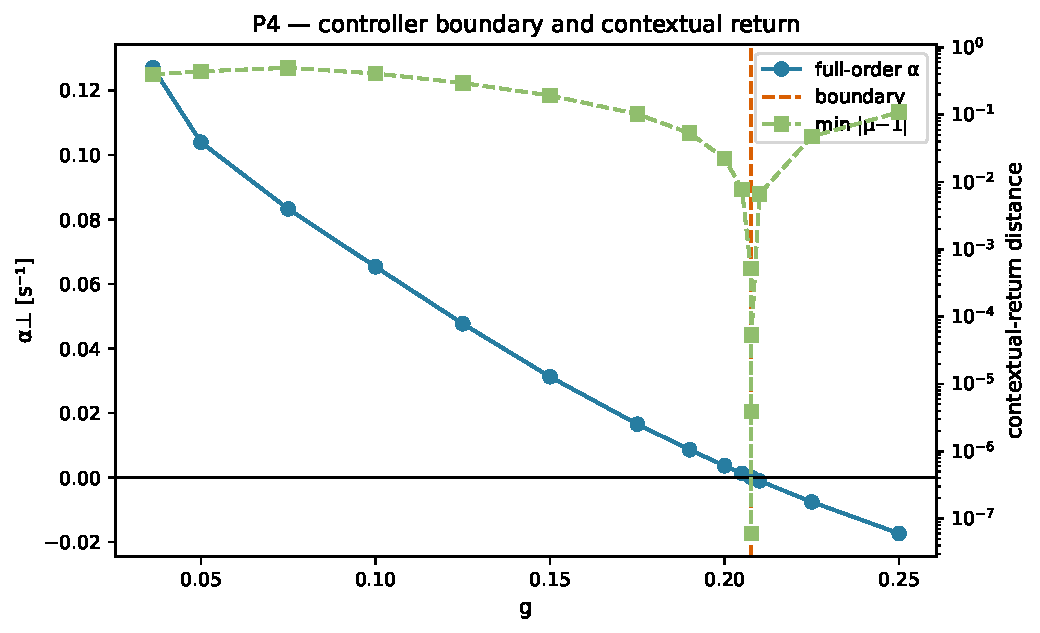
\includegraphics[width=.95\columnwidth]{../../../figures/tx4_blind_prediction/P4_alpha_return.pdf}
\caption{Full-order spectral abscissa and contextual-return boundary under the one-coordinate $g$ sweep.}
\label{fig:return}
\end{figure}

\section{Blind prediction}
The firewall allowed only the model, baseline network, local devices, and
port construction before reveal. The V4 predictor enumerated all 16 subsets:
15 stable predictions and one unstable H4 prediction. Full-order reveal gave
16/16, zero false-safe, zero false-unstable, exact H, and exact kappa=4.
The H4 reduced frequency was 0.622279671 Hz, agreeing with full order to
$1.4\times10^{-9}$ Hz.

The blind protocol was frozen before the reveal. It enumerated all 16 V4
subsets, wrote and hashed the prediction files, and only then loaded the
full-order answer tables. The V4 result is therefore an exact finite
pre-reveal prediction result; the later V9 run is a transfer stress test.

\begin{figure}[t]
\centering
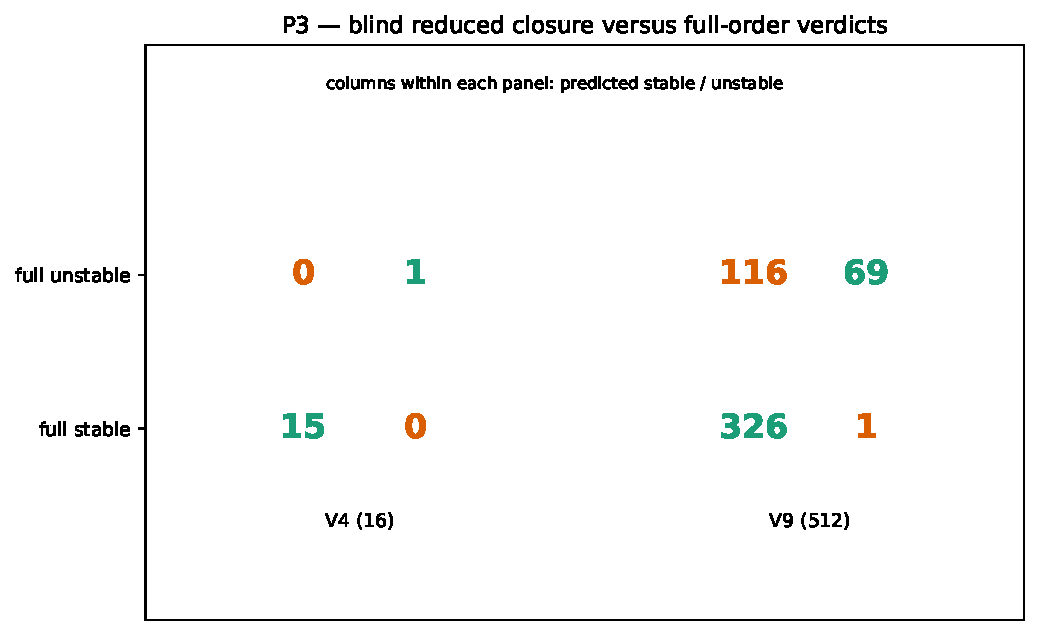
\includegraphics[width=.95\columnwidth]{../../../figures/tx4_blind_prediction/P3_blind_vs_full.pdf}
\caption{Blind V4 reduced-closure verdicts versus full-order reveal.}
\label{fig:blind}
\end{figure}

\section{Contextual mechanism}
For $R=H\setminus\{i\}$, define
$G_R=(I+Q_{RR})^{-1}$ and
$\mathcal R_{i|R}=Q_{iR}G_RQ_{Ri}$. Then
\begin{equation}
\det(I+Q_H)=\det(I+Q_{RR})\det(I-\mathcal R_{i|R}).
\end{equation}
At the boundary, the collective factor has singular value $2.2\times10^{-8}$
while local factors remain regular. The nearest contextual-return eigenvalue
is -0.999999965. The H4 controller boundary is $g=0.207681405$ in full order;
the reduced-only reproduction is 0.207681386. Its run timing was post-reveal,
so this agreement is reported with a procedural limitation.

At the boundary the local factor remains regular while the collective factor
approaches singularity. This is the mechanism-level distinction: the failure
is not attributed to a single isolated inverter pole. The factorization is
standard block algebra, and its empirical role here is to expose the
portfolio-conditioned return path.

\section{Controller and nonlinear validation}
Changing only $g$ to 0.25 gives $\alpha=-0.017385$ s$^{-1}$. Under the frozen
2\% bus-20 active-load pulse for 0.2 s, the proper subset is stable, H4 is
unstable, and retuned H4 is stable. Growth-sign agreement is 3/3. This is
nonlinear phasor-domain TDS, not EMT validation.

The common disturbance is a two-percent active-load pulse at bus 20 for
0.2 s. The three declared cases are a proper triple, H4 at the frozen
controller, and H4 after the fixed $g$ retuning. The estimated growth-rate
sign agrees with the linear alpha sign in all three cases. This supports the
ordering for the tested disturbance; it does not establish transient
security for arbitrary faults, pulses, or EMT representations.

\begin{figure}[t]
\centering
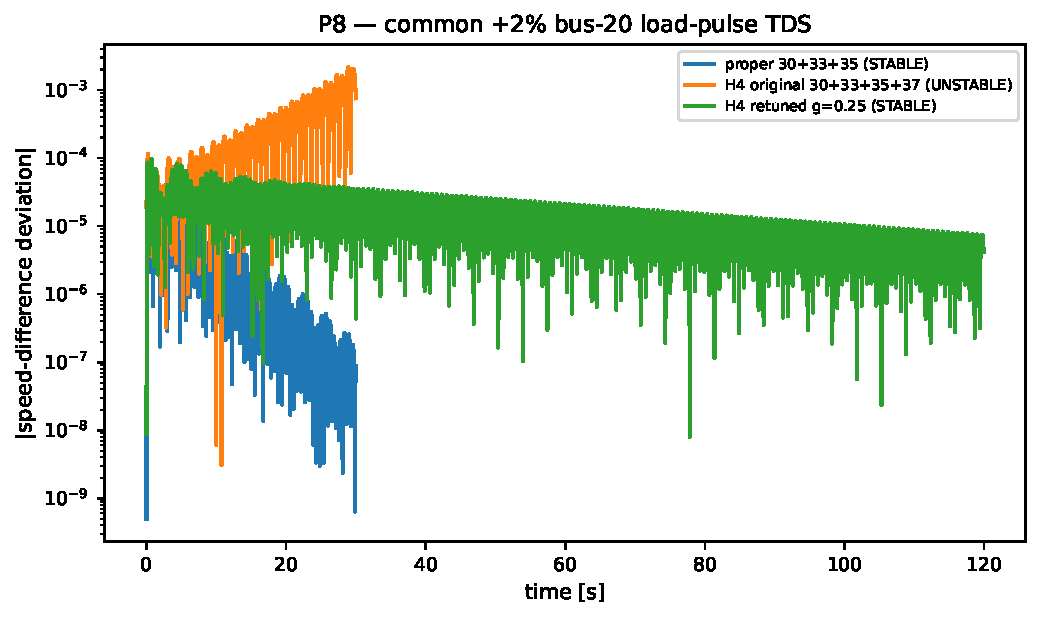
\includegraphics[width=.95\columnwidth]{../../../figures/tx4_blind_prediction/P8_TDS_final.pdf}
\caption{Common-disturbance nonlinear phasor-domain TDS for a proper subset, H4, and retuned H4.}
\label{fig:tds}
\end{figure}

\section{Aggregate counterexample and V9 limit}
The nearest fixed-rule V9 pair has six replacements and 0.2513\% normalized
MW/MVA mismatch: one portfolio is unstable ($\alpha=+324.249$) and the other
stable ($\alpha=-0.1664$). There is no exact aggregate match. Over all V9
subsets, accuracy is 395/512, false-safe count 116, false-unstable count 1,
and exact H recovery fails. Thus the predictive claim remains flagship-scoped.

The aggregate comparison reinforces the same caution. A fixed-rule,
same-cardinality V9 pair differs by only 0.2513\% in normalized MW/MVA
distance, yet one member is stable and the other unstable. This is not an
exact equal-penetration proof, because exact MW/MVA matching was unavailable;
it is a near-match counterexample against reading penetration as a sufficient
descriptor. Conversely, the V9 census has 116 false-safe cases, so the
reduced closure should not be marketed as an exact scalable classifier.

\begin{figure}[t]
\centering
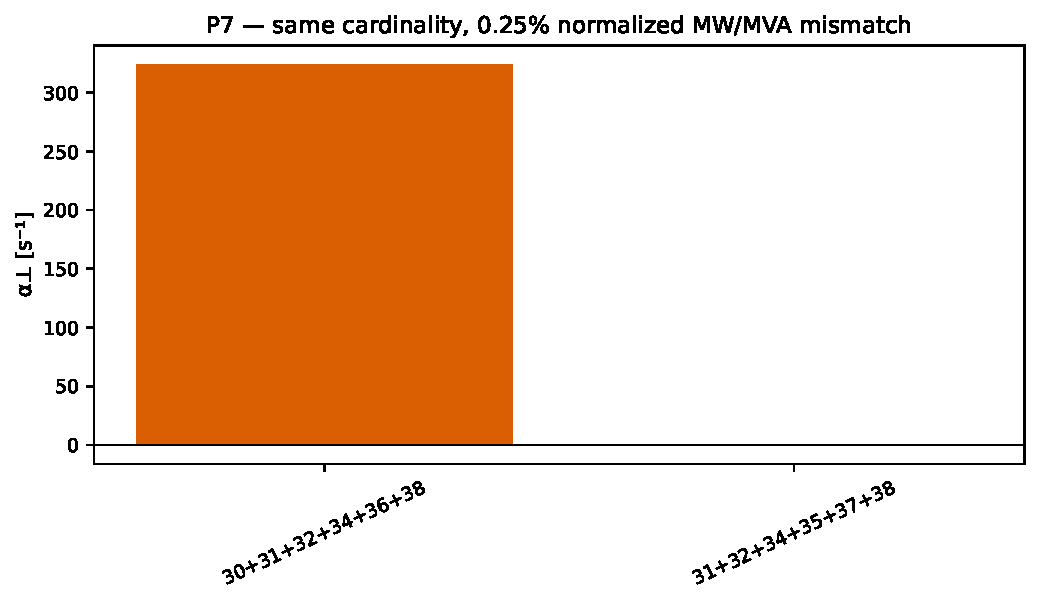
\includegraphics[width=.95\columnwidth]{../../../figures/tx4_blind_prediction/P7_aggregate_pair.pdf}
\caption{Near-matched aggregate replacement pair with opposite full-order verdicts.}
\label{fig:aggregate}
\end{figure}

\section{Discussion and limitations}
The critical mode is an inter-area electromechanical mode with network-
mediated converter participation; numerical residual and eigensolver checks
do not indicate an index pathology. The model is one IEEE-39 phasor-domain
implementation, ANDES support is limited, EMT remains unresolved, and the
reduced method is slower than full order. The value is diagnostic: it shows
what fails, why the collective closure fails, and how a fixed controller
coordinate moves the boundary.

\section{Conclusion}
The result supports the scoped statement: replacement safety is a portfolio
property in the frozen TX4 model, and a local-device/network closure can
predict the minimal four-bus failure before full simulation. Broader model
and network validation is required before a journal-level generalization.

\nocite{*}
\bibliographystyle{IEEEtran}
\bibliography{references}
\end{document}
